\documentclass{beamer}
\usepackage{amsmath}
\usepackage{amssymb}
\usepackage{physics}
\usepackage{amsthm}
\usepackage{graphicx}
\usepackage{caption}
\usepackage{subcaption}
\usepackage{listings}
\usepackage{units}
\usepackage{tensor}
\usepackage{accents}
\graphicspath{ {./figures/} }
\title{Aplikace spektrální metody}
\author{Dominika Hájková, Matyáš Fuksa, Ondřej Kureš}
\institute{Stormtrooperz}
\date{2021}

\begin{document}


\frame{\titlepage}
\begin{frame}
\frametitle{Spektrální metoda - Co to je?}
Byla nám dána obyčejná diferenciální rovnice
\begin{equation*}
\frac{1}{5}\frac{d^2u}{dx^2}+\frac{du}{dx}+u=f(x),
\end{equation*}
a musíme najít řešení u(x) na intervalu $(-1,1)$ s okrajovými podmínkami
\begin{align*}
\left. u \right|_{x=-1} &= \alpha, \\
\left. u' \right|_{x=1} &= \beta.
\end{align*}
Spektrální metodu použijeme takto: Místo, abychom řešili rovnici pro všechna $x \in (-1,1)$, budeme ji jen řešit pro určité interpolační body $\left\{ x_j \right\}_{j=1}^{N+2}$. Tyto interpolační body budou Čebyševovy body. 
\end{frame}

\begin{frame}
\frametitle{Spektrální metoda - Co to je? - pokračování}
\begin{equation*}
  \left(
    \frac{1}{5}
    \mathbb{D}_{\left(N + 2\right)\times \left(N + 2\right)}^2
    +
    \mathbb{D}_{\left(N + 2\right)\times \left(N + 2\right)}
    +
    \mathbb{I}_{\left(N + 2\right) \times \left(N + 2\right)}
  \right)
  \vec{u}_{N + 2}
  =
  \vec{f}_{N + 2}
  ,
\end{equation*}
\begin{equation*}
  \label{eq:55}
  \vec{u}_{N + 2}
  =_{def}
  \begin{bmatrix}
    u(x_1) \\
    u(x_2) \\
    u(x_3) \\
    \vdots \\
    u(x_{N + 1}) \\
    u(x_{N + 2})
  \end{bmatrix}
  ,
  \qquad
  \vec{f}_{N + 2} = _{def}
  \begin{bmatrix}
    f(x_1) \\
    f(x_2) \\
    f(x_3) \\
    \vdots \\
    f(x_{N + 1}) \\
    f(x_{N + 2})
  \end{bmatrix}
\end{equation*}
\end{frame}

\begin{frame}[fragile]
\frametitle{Trám na jiný způsob - Kód}
\begin{lstlisting}[language=Matlab, basicstyle=\small, numbers=left,breaklines=true]
f = @(x) 75*9.81*exp(-x.^2/(2*0.01)); alpha = 0; beta = 0; gama = 0 ;delta = 0; n = 18; E = 9.4*10^6; Izz = 3;l = 10;X = [-l/2,l/2];
L = E*Izz*diffmat([n n+4],4,X);
vT = diffrow(n+4,0,-l/2,X); wT = diffrow(n+4,0,l/2,X); uT = diffrow(n+4,1,-l/2,X); sT = diffrow(n+4,1,l/2,X);
A = [L; vT; wT; uT; sT];
rhs = [gridsample(f,n); alpha; beta; gama; delta];
u = A\rhs;
tiledlayout(2,1)
nexttile
plot(chebfun(-u,X),'.-');ylim([-1 1]);
nexttile
plot(chebfun(-u,X),'.-');ylim([-0.001 0.001])
\end{lstlisting}
\end{frame}

\begin{frame}
\frametitle{Trám na jiný způsob - Obrázky}
\centering
\begin{figure}
\includegraphics[width=.9\linewidth]{První.png}
\includegraphics[width=.9\linewidth]{Druhý.png}
\caption{Musím doplnit}
\end{figure}
\end{frame}

\begin{frame}
\frametitle{Kmitání membrán - Analytický rozbor}
\pause
Máme rovnici $\Delta u=-\lambda u$. Jelikož pracujeme na oblasti obdelníka, můžeme $u(x,y)$ přepsat do nového tvaru: $u(x,y)=X(x) Y(y)$.
\pause
Dostáváme novou rovnici:
\begin{equation}
   \frac{\partial^2 X}{\partial x^2} Y
      + X \frac{\partial^2 Y}{\partial y^2}=-\lambda X Y
\end{equation}
\pause
Provedeme sérii úprav, které nás dovedou na systém dvou rovnic. Vyřešením soustavy dostaneme obecné řešení pro $X(x)$ a $Y(y)$.
\pause
\begin{subequations} 
\begin{equation}
X(x)=A_1 \sin{(\sqrt{\lambda-\alpha}x)}+B_1 \cos{(\sqrt{\lambda-\alpha}x)}
\end{equation}
\begin{equation}
Y(y)=A_2 \sin{(\sqrt{\alpha}y)}+B_2 \cos{(\sqrt{\alpha}y)}
\end{equation}
\end{subequations}

\end{frame}

\begin{frame}
\frametitle{Kmitání membrán - Analytický rozbor - pokračování}
Použitím Dirichletových okrajových podmínek ($X(0)=X(a)=0$ a $Y(0)=Y(b)=0$, kde $a$ je šířka a $b$ je výška obdélníku), získáme vlastní číslo

\begin{equation}
\lambda_{m,n}=\frac{m^2\pi^2}{a^2}+\frac{n^2\pi^2}{b^2}
\end{equation}
\pause
a vlastní vektor
\begin{equation}
u(x,y)_{m,n}=A\sin{(\frac{m\pi}{a}x)}\sin{(\frac{n\pi}{b}y)},
\end{equation}
kde $m$,$n$ jsou přirozená čísla.
\end{frame}



\begin{frame}
\frametitle{Kmitání membrán - Výsledky 1. část}
\centering
\begin{figure}
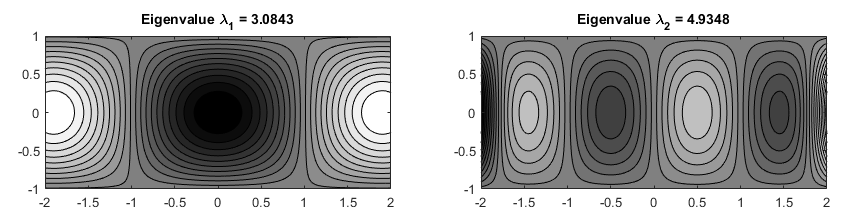
\includegraphics[width=1\linewidth]{obdelnicky1.png}
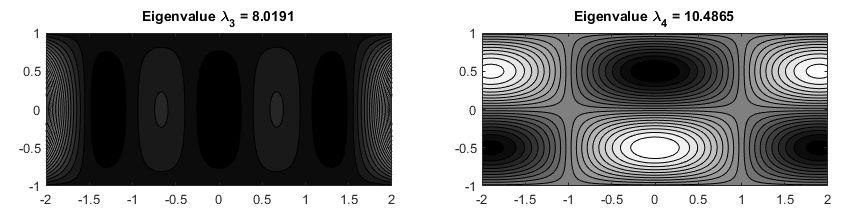
\includegraphics[width=1\linewidth]{obdelnicky2.png}
\caption{Získáno v Matlabu}
\end{figure}
\end{frame}

\begin{frame}
\frametitle{Kmitání membrán - Výsledky 2. část}
\centering
\begin{figure}
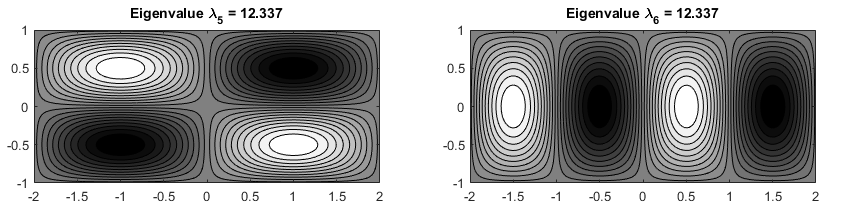
\includegraphics[width=1\linewidth]{obdelnicky3.png}
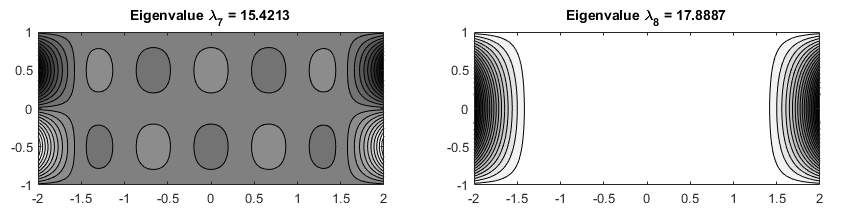
\includegraphics[width=1\linewidth]{obdelnicky4.png}
\caption{Získáno v Matlabu}
\end{figure}
\end{frame}

\begin{frame}
\frametitle{Kmitání membrán - Výsledky 3. část}
\centering
\begin{figure}
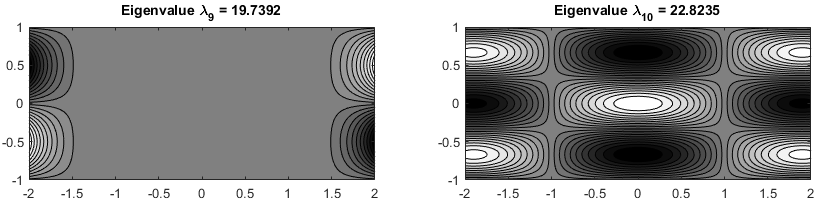
\includegraphics[width=1\linewidth]{obdelnicky5.png}
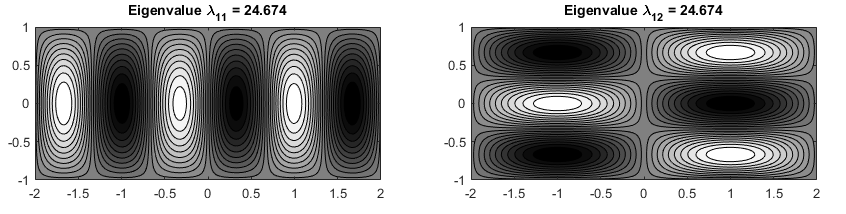
\includegraphics[width=1\linewidth]{obdelnicky6.png}
\caption{Získáno v Matlabu}
\end{figure}
\end{frame}

\begin{frame}
\frametitle{Kmitání membrán - Výsledky 4. část}
\centering
\begin{figure}
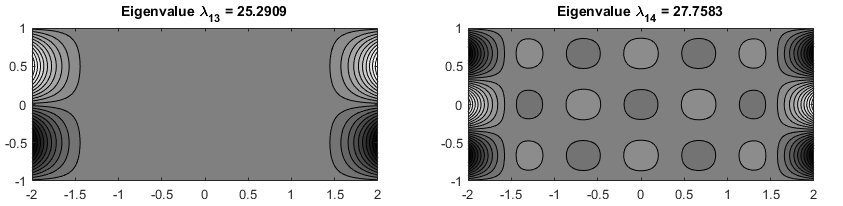
\includegraphics[width=1\linewidth]{obdelnicky7.png}
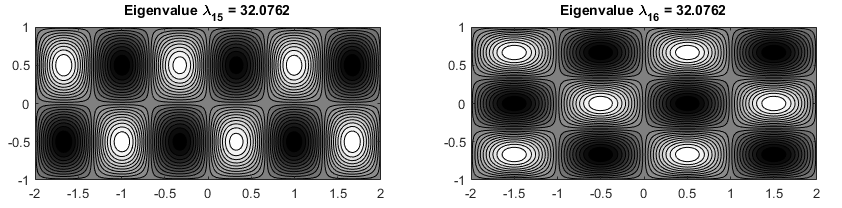
\includegraphics[width=1\linewidth]{obdelnicky8.png}
\caption{Získáno v Matlabu}
\end{figure}
\end{frame}

\begin{frame}
\frametitle{Kmitání membrán - Výsledky 5. část}
\centering
\begin{figure}
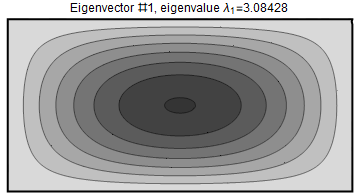
\includegraphics[width=.6\linewidth]{rectangle-eigenvector-1.png}
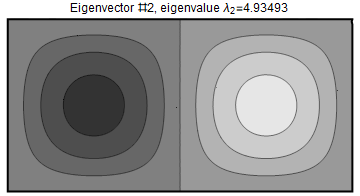
\includegraphics[width=.6\linewidth]{rectangle-eigenvector-2.png}
\caption{Získáno v Mathematice}
\end{figure}
\end{frame}

\begin{frame}
\frametitle{Kmitání membrán - Výsledky 6. část}
\centering
\begin{figure}
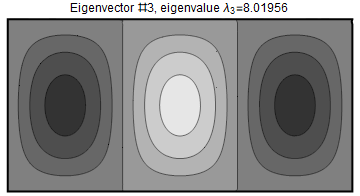
\includegraphics[width=.6\linewidth]{rectangle-eigenvector-3.png}
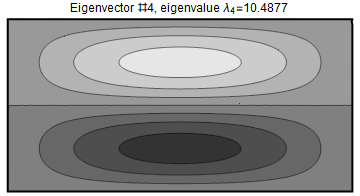
\includegraphics[width=.6\linewidth]{rectangle-eigenvector-4.png}
\caption{Získáno v Mathematice}
\end{figure}
\end{frame}

\begin{frame}
\frametitle{Kmitání membrán - Výsledky 7. část}
\centering
\begin{figure}
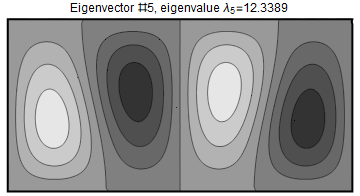
\includegraphics[width=.6\linewidth]{rectangle-eigenvector-5.png}
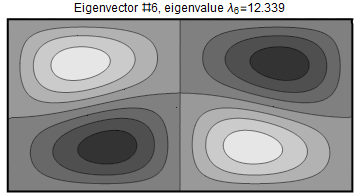
\includegraphics[width=.6\linewidth]{rectangle-eigenvector-6.png}
\caption{Získáno v Mathematice}
\end{figure}
\end{frame}

\begin{frame}
\begin{center}
\begin{huge}
Děkujeme za pozornost
\end{huge}
  \centering
  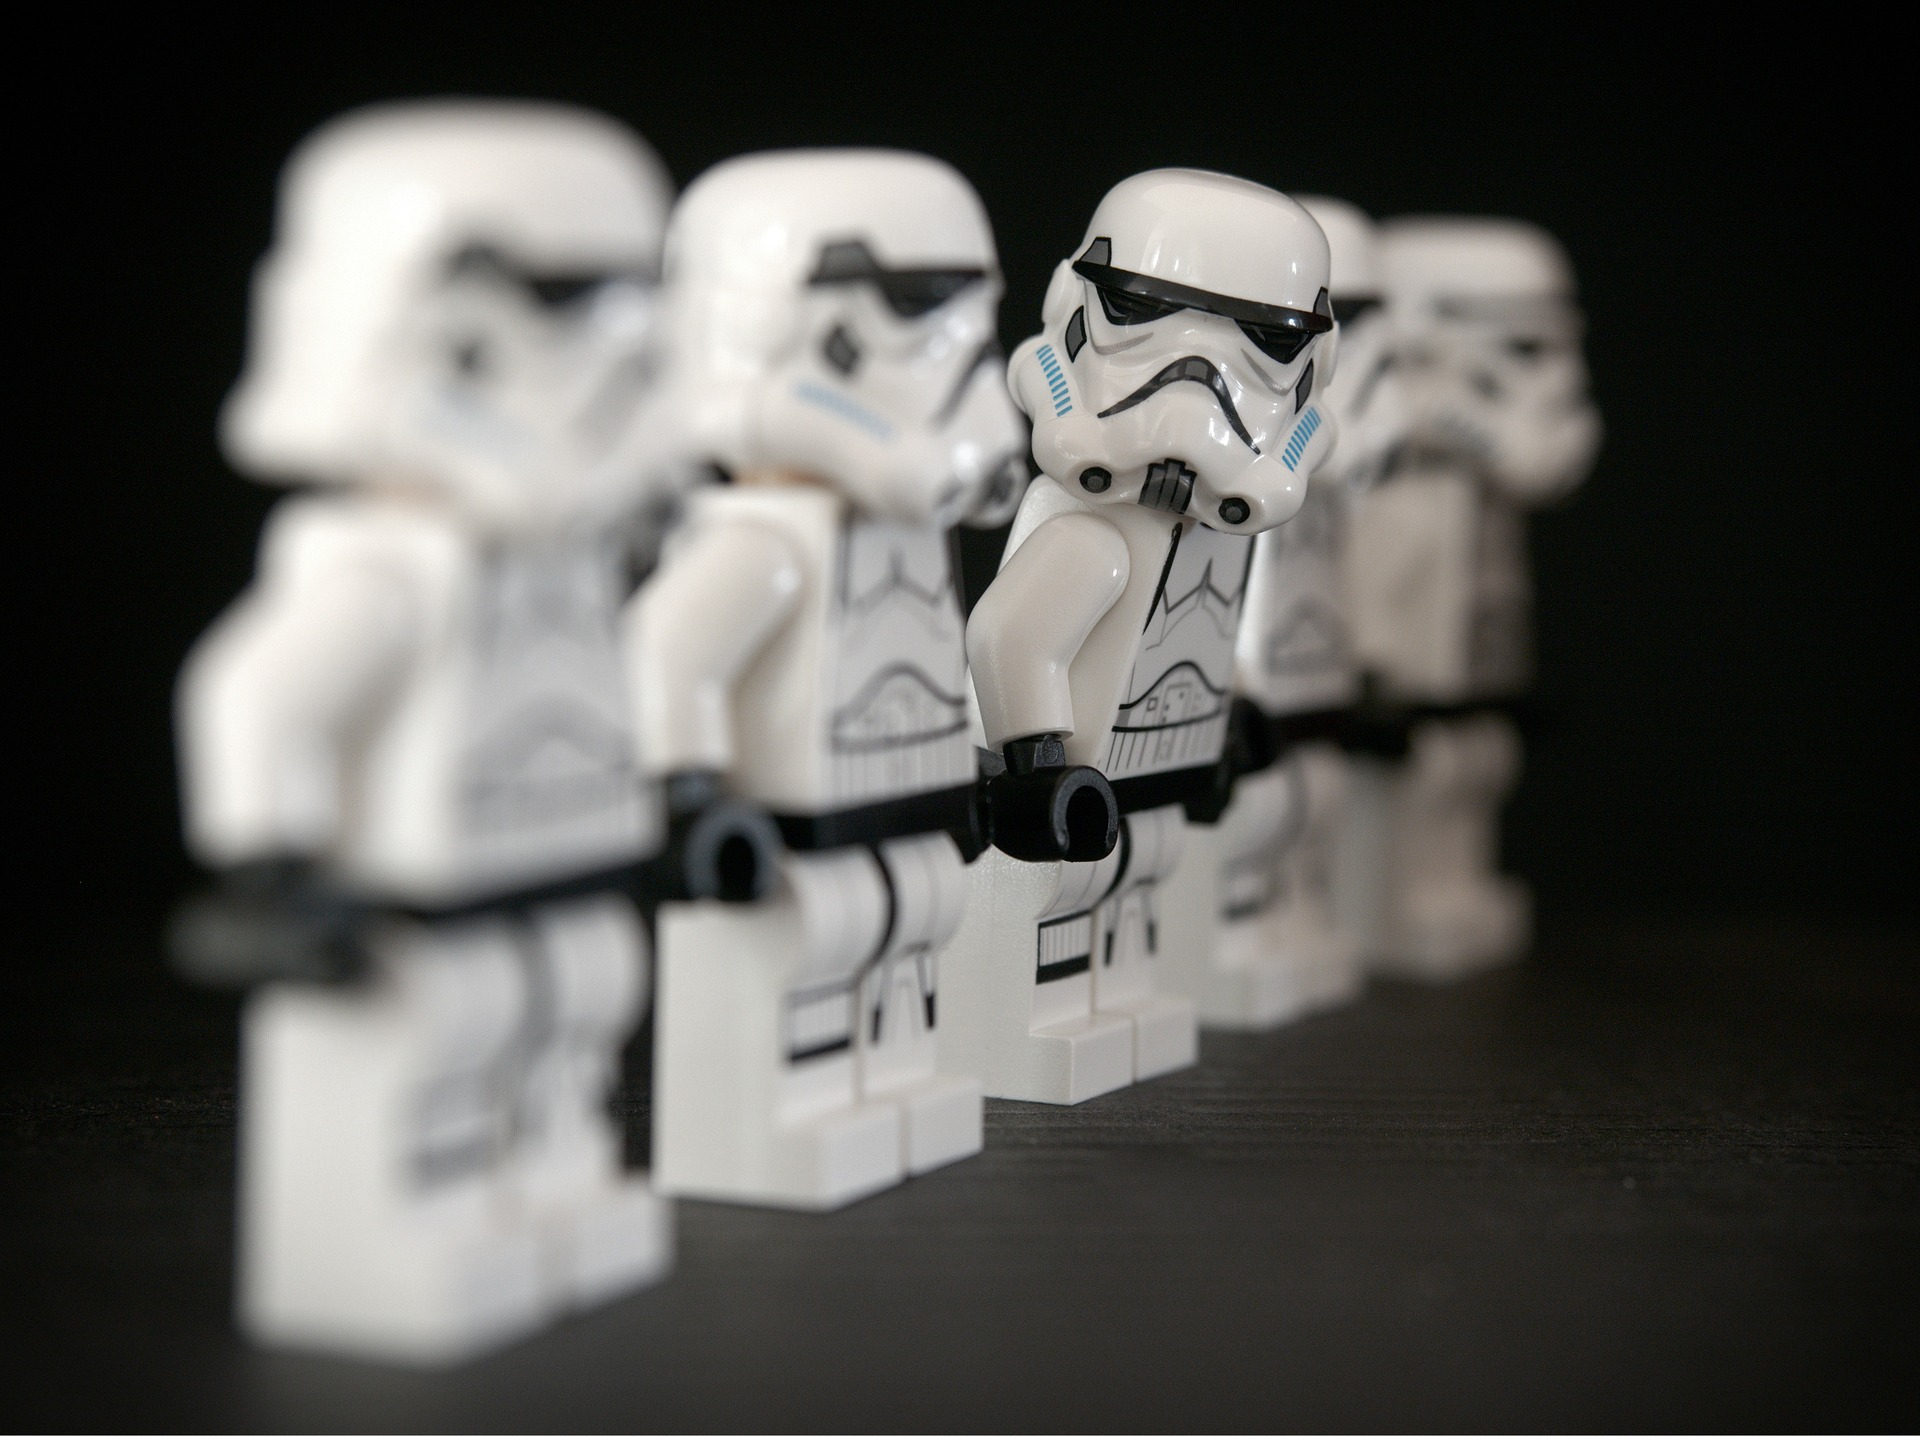
\includegraphics[width=.8\linewidth]{stormtroop.jpg}
\end{center}

\end{frame}
\end{document}